\documentclass{book}
\usepackage[utf8]{inputenc}
\usepackage{graphicx}
\usepackage{hyperref}

%\title{CW-test}
%\author{melika derakhshani}
%\date{April 2021}

\begin{document}
\tableofcontents
This is a test document! \hspace{1cm} testtest

%\maketitle
\newpage
\chapter{Introduction}

\section{Test}
Table \ref{tab:table1} ....

List of courses:
\begin{enumerate}
    \item OS
    \item AP
    \item Network
    \item CW
    \begin{itemize}
        \item Introduction
        \item MSWord
        \item MSPPT
        \item Web Programming
        \item Latex
    \end{itemize}
\end{enumerate}
\subsection{History}
\subsubsection{Before 2000}
CW class
\begin{table}[h]
    \centering
    \begin{tabular}{|c|c|c|}
         \hline
         Firstname & Lastname & Age \\
         \hline
         Samaneh   & Emami    & 34 \\
         \hline
    \end{tabular}
    \caption{Teacher Information}
    \label{tab:table1}
\end{table}

\newpage
\begin{figure}[t]
    \centering
    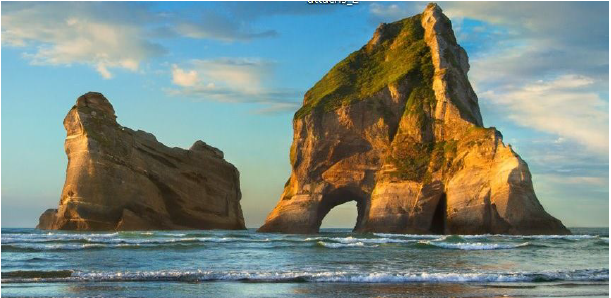
\includegraphics[width=\textwidth]{Capture.PNG}
    \caption{The Sea}
    \label{fig:sea}
\end{figure}
\subsubsection{After 2000}
\begin{equation}
    y = \frac{a + b}{\sqrt{c-d}}
    \label{eq:equation1}
\end{equation}

\subsection{Motivation}
$\beta$
\newpage

\chapter{Related Works}
\begin{equation}
    \alpha = \sum_{i=0}^{i=n}
    \label{eq:eqation2}
\end{equation}

Equation \ref{eq:equation1} shows that ....

Figure~\ref{fig:sea} refers to ....
\end{document}
